\subsection{Entwurf der Applikationsarchitektur}
\label{subsec:entwurf-der-applikationsarchitektur}


Der Entwurf der Applikationsarchitektur bildet die konzeptionelle Grundlage für die technische Umsetzung der entwickelten Web-Applikation.
Das Ziel ist es, eine Struktur zu schaffen, die modular, wartbar und erweiterbar ist und die gleichzeitig den funktionalen Anforderungen gerecht wird und sich in die bestehende Systemlandschaft integrieren lässt.
Die Architektur der Anwendung ist schichten- und komponentenorientiert aufgebaut und nutzt das Webframework Flask, welches eine klare Trennung zwischen der Präsentations-, Logik- und Datenhaltungsschicht ermöglicht.


\subsubsection{Architekturübersicht}
\label{subsubsec:arch}
Die Applikation soll als serverbasierte Webanwendung im Client-Server-Modell funktionieren.
Das bedeutet: Während der Server die Datenverarbeitung, -speicherung und -bereitstellung übernimmt, ermöglicht der Client über den Webbrowser die Darstellung und Interaktion.
Die Anwendung ist in mehrere Schichten gegliedert, zu denen man die einzelnen Programmteile zuordnen kann.
Die Anwendung wird in folgende Schichten gegliedert:

\begin{itemize}
\item Präsentationsschicht (Frontend): Bereitstellung der Benutzeroberfläche über HTML-Templates, CSS und JavaScript.

\item
Applikationslogik (Backend): Implementierung der Geschäftslogik, Steuerung des Datenflusses und Verarbeitung der XML-Dateien.

\item
Datenhaltungsschicht: persistente Speicherung der extrahierten Mess- und Gerätedaten in einer relationalen Datenbank mittels ORM.

\end{itemize}

Ein schematisches Architekturdiagramm dieser Struktur ist in Abbildung \ref{fig:arch_minimal} dargestellt.

\begin{figure}[H]
    \centering
    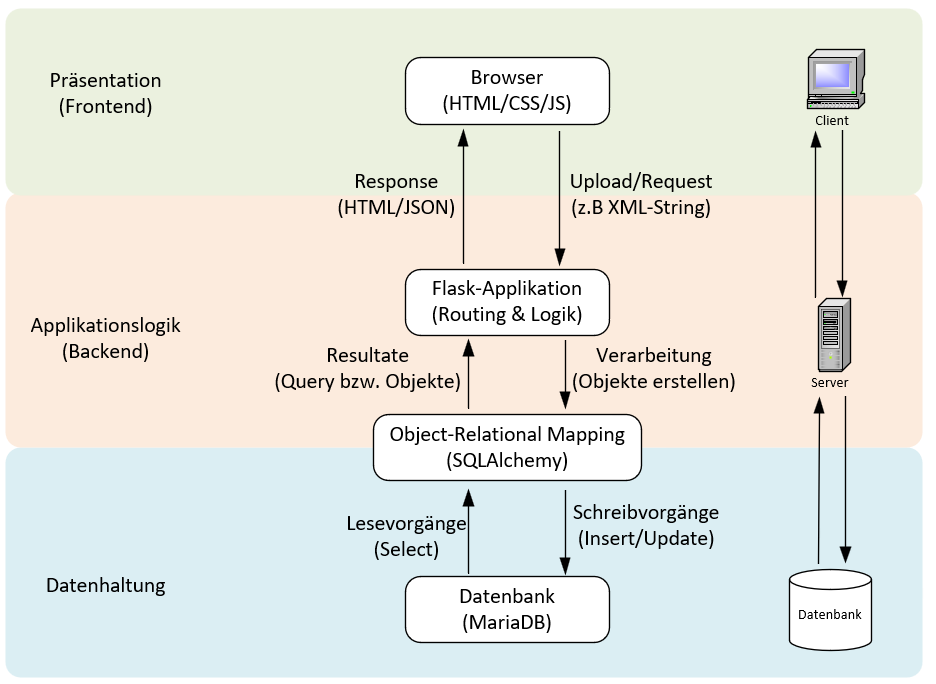
\includegraphics[width=0.95\textwidth]{Grafiken/Architekturdiagramm}
    \caption{Schematisches Architekturdiagramm der Applikation}
    \label{fig:arch_minimal}
    {Quelle: Eigene Darstellung mit Microsoft Visio}
\end{figure}

Der Entwurf der Ordnerstruktur für die Applikation wird in Abbildung \ref{fig: Grundlegende Ordnerstruktur der Applikation} dargestellt.

\begin{figure}[H]
    \centering
    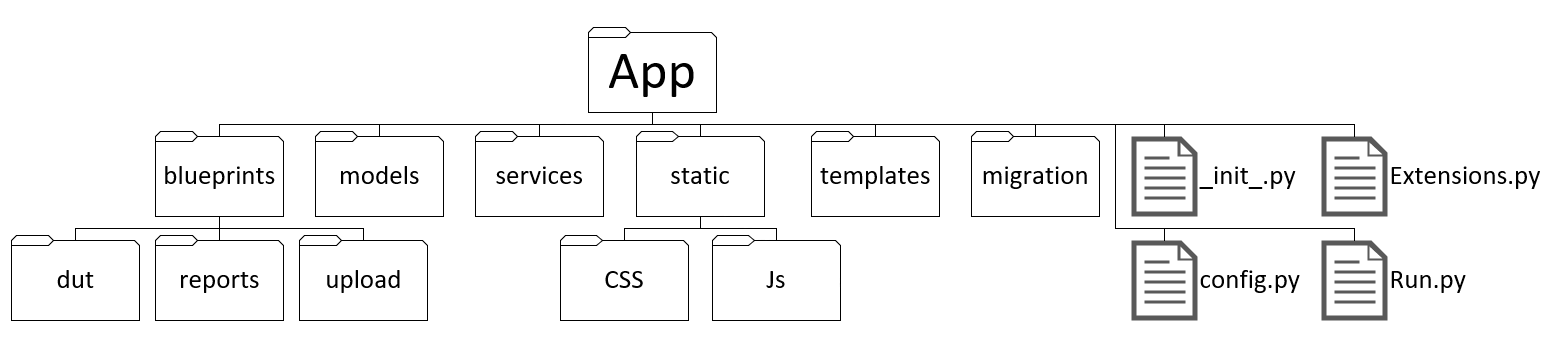
\includegraphics[width=1\textwidth]{Grafiken/Minimale Ordnerstruktur Projekt}
    \caption{Grundlegende Ordnerstruktur der Applikation}
    \label{fig: Grundlegende Ordnerstruktur der Applikation}
    {Quelle: Eigene Darstellung mit Microsoft Visio}
\end{figure}

\subsubsection{Präsentationsschicht}


Die Präsentationsschicht besteht aus einer Kombination aus HTML-Templates und statischen Ressourcen (CSS, JavaScript),
die im Verzeichnis templates/ bzw. static/ abgelegt werden.

\begin{itemize}

\item
Die Templates für die einzelnen Seiten der Applikation für das Hochladen, die Darstellung der sich in der Datenbank befindenden Berichte
und grafische Darstellungen bilden den Kern der Weboberfläche.

\item
Statische Dateien wie CSS-Stylesheets und das JavaScript für die Erstellung der Graphen dienen der Gestaltung und der
interaktiven Darstellung von Messergebnissen.

Die Kommunikation mit der Logikschicht erfolgt über die definierten Flask-Blueprints, die als modulare Controller agieren.

\end{itemize}

\subsubsection{Applikationslogik}

Die zentrale Geschäftslogik ist in modularen Blueprints und Servicekomponenten realisiert.

Die drei Blueprints \code{upload}, \code{reports} und \code{dut} kapseln die jeweiligen Funktionsbereiche:

\begin{itemize}

\item
upload: Einlesen und Validieren von XML-Dateien.

\item
dut: Verarbeitung und Anzeige der Daten eines „Device Under Test“.

\item
reports: Zusammenstellung und Ausgabe von Auswertungen.

\end{itemize}

Unterstützt werden diese durch das Modul in dem Ordner services/, das die eigentliche Logik zur Datenverarbeitung bereitstellt.
Dieser Ordner soll Dateien für folgende Aufgaben beinhalten:

\begin{itemize}

\item
Eine Datei für das Übernehmen des Parsens und Einlesens der XML-Daten.

\item
Eine Datei für vordefinierte Datenbankabfragen.

\item
Eine Datei für Hilfsfunktionen, z. B. zur Zeitreihenanalyse und Datenaufbereitung.

\item
Eine Datei dient der Erstellung und Formatierung von Report-Daten für die grafische Darstellung.

\end{itemize}

Die Applikationslogik soll über die Datei \code{run.py} initialisiert werden, welche den Flask-Server startet und die Anwendungskonfiguration aus \code{config.py} einliest.


\subsubsection{Datenhaltungsschicht}

Die Datenhaltung soll über ein relationales Datenbanksystem erfolgen, das über das Flask-eigene SQLAlchemy \ac{ORM} angebunden ist.
Dabei sollen die Datenmodelle im Verzeichnis models/ definiert werden und die logischen Entitäten der Prüfanlage abbilden.
Die Dateien werden nach den Tabellen in Abbildung \ref{fig: Darstellung der Datenbanktabellen und ihrer Verbindungen} unterteilt.
Außerdem sollen die Beziehungen zwischen den Modellen ermöglichen, dass eine strukturierte und relationale Abbildung der Prüfdaten dargestellt wird.
Wodurch eine effiziente Abfrage und Analyse möglich ist.

Für die Migrationen werden mit der Bibiothek \code{Flask-Migration} verwaltet, wodurch das Verzeichnis \code{migrations} zustande kommen soll.






























